%\documentclass[11pt,a4paper,twoside]{tesis}
% SI NO PENSAS IMPRIMIRLO EN FORMATO LIBRO PODES USAR
\documentclass[11pt,a4paper]{tesis}
\setcounter{tocdepth}{3}
\setcounter{secnumdepth}{3}

\usepackage{graphicx}
\usepackage[utf8]{inputenc}
\usepackage[spanish]{babel}
\usepackage{biblatex}
\usepackage{csquotes}
\usepackage{fancyhdr}
\usepackage{amsmath}
\usepackage{amssymb}

\setlength{\marginparwidth}{2cm}
\setlength{\headheight}{15pt}

\usepackage{todonotes}

\usepackage[left=3cm,right=3cm,bottom=3cm,top=3cm]{geometry}


% Bibliography
\addbibresource{tesis.bib}

% Glossary
\usepackage[acronym]{glossaries}
\makeglossaries
\newglossaryentry{domain-knowledge}{%
	name={domain knowledge},%
	description={valid knowledge used to refer to an area of human endeavour, an autonomous computer activity, or other specialized discipline}}

%batch/ambiente batch
%streaming/ambiente streaming
%framework
%feature
%mineria de datos
%aprendizaje automatico
% inteligencia artificial
% árboles de decisión
%naive bayes
% procesamiento de lenguaje natural
% meka
% weka
%cidetic
% clustering
% python
% java

\newacronym{mll}{MLL}{Clasificación multi-etiquetas}
\newacronym{moa}{MOA}{Massive Online Analysis}
\newacronym{ia}{IA}{Inteligencia Artificial}
\newacronym{ti}{TI}{Tecnología de la Información}
\newacronym{id3}{ID3}{Iterative Dichotomiser 3}
\newacronym{cart}{CART}{Classification and Regression Tree}
\newacronym{br}{BR}{Binary Relevance}
\newacronym{cc}{CC}{Classifier Chains}
\newacronym{lp}{LP}{Label Powerset}
\newacronym{lc}{LC}{Label Combination}
\newacronym{ebr}{EBR}{Ensamble de Binary Relevance}
\newacronym{ecc}{ECC}{Ensamble de Classifier Chains}
\newacronym{ps}{PS}{Pruned Set}
\newacronym{ht}{HT}{Hoeffding Tree}
\newacronym{mlht}{MLHT}{Multi-label Hoeffding Tree }
\newacronym{isoup}{iSoup-Tree}{Incremental Structured Output Prediction Tree}
\newacronym{rtg}{RTG}{Generador de Árbol Aleatorio}
\newacronym{rbf}{RBF}{Generador de Función Radial Base}
\newacronym{vp}{VP}{Verdaderos Positivos}
\newacronym{vn}{VN}{Verdaderos Negativos}
\newacronym{fp}{FP}{Falsos Positivos}
\newacronym{fn}{FN}{Falsos Negativos}
\newacronym{efmp}{EFMP}{Ensamble Fijo por Mayoría Ponderada}
\newacronym{efmp2}{EFMP2}{Ensamble Fijo por Mayoría Ponderada 2}
\newacronym{dwm}{DWM}{Dynamic Weighted Majority}
\newacronym{gooweml}{GOOWE-ML}{GOOWE-ML}
\newacronym{cidetic}{CIDETIC}{Centro de Investigación, Docencia y Extensión en TIC de la Universidad Nacional de Luján}



\begin{document}

%%%% CARATULA
\def\titulo{Licenciado }

\def\autor{Juan Cruz Cardona}
\def\tituloTesis{Clasificación de flujos de datos continuos y multi etiquetados}
\def\runtitulo{Clasificación de flujos de datos continuos y multi etiquetados}
\def\runtitle{Clasificación de flujos de datos continuos y multi etiquetados}
\def\director{Santiago Banchero}
\def\fecha{2021}

\newcommand{\HRule}{\rule{\linewidth}{0.2mm}}
%
\thispagestyle{empty}

\begin{center}\leavevmode

\vspace{-2cm}

\begin{tabular}{l}

\includegraphics[width=5cm]{img/logo_unlu}
\end{tabular}

{\large \sc Universidad Nacional de Luján}

\vspace{5.0cm}

{\huge\bf \tituloTesis}

\vspace{2cm}

{\large Tesina de grado presentada para optar al t\'{\i}tulo de\\
\titulo en Sistemas de Informaci\'on}

\vspace{2cm}

{\Large \autor}

\end{center}

\vfill

{\large

{Director: \director}

\vspace{.2cm}

\begin{center}
\fecha
\end{center}
}

\newpage\thispagestyle{empty}


%%%% ABSTRACTS, AGRADECIMIENTOS Y DEDICATORIA
\frontmatter
\pagestyle{empty}
%\begin{center}
%\large \bf \runtitulo
%\end{center}
%\vspace{1cm}
\chapter*{\runtitulo}

\noindent La clasificación multi-etiquetas es un paradigma de aprendizaje
supervisado que generaliza las técnicas clásicas de clasificación para abordar
problemas en donde cada instancia de una colección se encuentra asociada a
múltiples etiquetas. La mayor parte de los trabajos de investigación han sido
realizados en contextos de aprendizaje por \textit{batch}. Los ambientes de
flujo continuo de datos  (o \textit{streaming}) presentan nuevos desafíos a esta
área debido a las limitaciones de tiempo de respuesta y almacenamiento que
acarrean. En la presente investigación se aplican algoritmos de clasificación
multi-etiquetas a colecciones estructuradas y no estructuradas. Los experimentos
se llevaron a cabo en ambientes simulados de \textit{streaming} de datos para
conocer el impacto que produce este contexto sobre los resultados de la
clasificación y acoplar el modelo a escenarios del mundo real. A su vez, se
partió de estas colecciones de datos para generar instancias sintéticas y así
producir flujos potencialmente infinitos. A este fin se presenta un método de
generación de instancias sintéticas que busca replicar fenómenos particulares de
colecciones multi-etiquetadas. Por último, se diseña una estrategia de ensambles
de algoritmos, \acrshort{efmp}, en búsqueda de una mejora en la calidad de la
tarea de predicción de objetos no observados por el modelo. De esta manera, se
provee a la comunidad de nuevos estudios experimentales sobre algoritmos y
colecciones ya conocidos del área de clasificación multi-etiquetas, de manera
tal de extender el conocimiento sobre su rendimiento bajo escenarios evolutivos
y de naturaleza variable.

\bigskip

\noindent\textbf{Palabras claves:} clasificación, multi-etiquetas, \textit{streaming}, algoritmos, flujos.


%\cleardoublepage
%\chapter*{Agradecimientos}

\noindent En el tiempo que llevó realizar esta tesis he recibido el apoyo y
asistencia de mucha gente y quiero aprovechar este espacio para reconocerlo.

Me gustaría agradecer en primer lugar a mi director, Santiago Banchero, quien
con su conocimiento y experiencia me ha guiado por cada una de las etapas de este
proceso. Su perseverancia y compromiso desde el inicio ha sido esencial para
encauzar este proyecto y ha logrado sacar lo mejor de mí en el proceso.

Además,s agradezco al Centro de Investigación, Docencia y Extensión en TIC de la
Universidad Nacional de Luján (CIDETIC) por proveer los recursos humanos y
computacionales necesarios para este proyecto. No hubiese podido arribar a estos
resultados de no haber sido por el soporte por ellos recibido.

También quiero agradecer especialmente a mi familia, por el sostén emocional a
lo largo de este proceso y por confiar en mí, en las buenas y en las malas.
Gracias a mis padres, a mis hermanas y a mi abuela Lucía.  Finalmente, este
objetivo no se hubiera cumplido sin el apoyo incondicional de mis amigos,
quienes estuvieron junto a mí y supieron entender mis ausencias. Incluso se han
tomado el tiempo de leer los esbozos del escrito, participar en exposiciones o
compartir charlas conmigo, y eso es un privilegio. Por eso gracias Lucas, Luz,
Vicky, Mica, Torne y Alan.
 % OPCIONAL: comentar si no se quiere

% \cleardoublepage
% \hfill \textit{A L. C.}
  % OPCIONAL: comentar si no se quiere

\cleardoublepage
\tableofcontents

\mainmatter
\pagestyle{fancy}

%%%% ACA VA EL CONTENIDO DE LA TESIS
\chapter{Introducción}

\section{Fundamentos}

En los últimos años ha habido un aumento considerable de datos de diversa índole
y generados por fuentes heterogéneas. Según los autores
\citeauthor{gantz_extracting_2011}, el volumen total de datos creados y
replicados en el mundo durante el año 2011 supera los 1.8 ZB (zettabytes) y se
ha estimado que duplica cada dos años \cite{gantz_extracting_2011}. Los avances
en el área de tecnología de la información (IT) han contribuido a una continua
producción de datos y expansión del campo digital, tal es el caso para la red
social \textit{Facebook}, la cual recibe cada hora un flujo de 10 millones de
fotos que publican sus usuarios \cite{mayer-schonberger_big_2013}. A estas
grandes colecciones de datos se las conoce como \textit{big data} y acarrean
nuevas oportunidades y desafíos al campo de las ciencias de la computación. En
cuestiones económicas, un análisis a gran escala en búsqueda de tendencias en el
comportamiento de los usuarios o clientes de un sistema puede dar una ventaja
competitiva en el mercado y, en adición, proveer de un servicio valioso a la
comunidad. Potencialmente, la \textit{big data} puede ser una fuente que
proporcione a la comunidad de conocimiento nuevo sobre el mundo en el que
habita, o como ha mencionado \citeauthor{fayyad_advances_1996} en su escrito
sobre el descubrimiento de conocimiento, “Los datos que percibimos de nuestro
ambiente son la evidencia básica que usamos para construir teorías y modelos
sobre el universo en el que vivimos”\footnote{“Data we capture about our
   environment are the basic evidence we use to build theories and models of the
universe we live in” \cite[p. 2]{fayyad_advances_1996}. Traducción propia.}.

Sin embargo, volúmenes masivos de datos tornan obsoletos los tradicionales
métodos manuales de análisis de datos y surge la necesidad de desarrollar
técnicas automatizadas para extraer patrones en los datos y obtener
conocimiento. Con este fin, se han desarrollado técnicas en las áreas de minería
de datos y aprendizaje de máquinas que abordan estas colecciones en búsqueda de
conocimiento válido y útil. Dichas técnicas se han enfocado en el aprendizaje
por \textit{batch} \cite{gama_knowledge_2010}, lo que significa que el algoritmo
dispone de la colección completa, almacenada en disco, y con la cual genera un
modelo a partir de una o múltiples iteraciones sobre todos los datos. No
obstante, el aprendizaje por \textit{batch} trae aparejada una dificultad en su
misma definición: requiere de todos los datos de la colección presentes y
accesibles en todo momento,  lo cual no siempre es posible. Además se suma una
limitante que es clave en el contexto actual de alta disponibilidad de datos:
hoy en día una buena parte de los datos generados proviene de flujos continuos o
‘\textit{streamings}’ de datos \cite{bifet_big_2014}. Estos flujos son
potencialmente ilimitados, arriban de a una instancia por vez, y son analizados
con restricciones altas de tiempo de procesamiento y de memoria.  Tal es el caso
para aplicaciones de sensores, monitoreo de redes y administración de tráfico,
flujo de clics de un usuario en la web, redes sociales, entre otros.  Los
algoritmos de aprendizaje que actúen en este entorno dinámico deben contar con
mecanismos que permitan manejar cambios en la naturaleza o distribución de los
datos, tanto para incorporar datos nuevos, como para descartar los datos
antiguos. Por estas razones, se torna necesario que las aplicaciones basadas en
clasificación en tiempo real adapten sus operaciones de entrenamiento y
predicción para lograr mejores resultados \cite{sousa_multi-label_2018}.

Dentro del área de minería de datos, una de las principales tareas es la de
clasificación, la cual consiste en entrenar un modelo que sea capaz de asignar
una única etiqueta a una instancia desconocida. No obstante, existen problemas
de clasificación en donde múltiples etiquetas son necesarias para caracterizar
una instancia. Por ejemplo, una noticia de diario referida al accidente aéreo
que sufrió el plantel de fútbol del club Chapecoense puede ser clasificado en la
categoría de “Fútbol” tanto como en la de “Tragedias”. Del mismo modo, un video
documental sobre la vida de Borges puede anotarse como “Biografía”, “Literatura”
o incluso “Buenos Aires” si se mostraran imágenes de la ciudad. Este tipo de
problemas es llamado \acrfull{mll} \footnote{Siglas provenientes de su
abreviación en inglés, Multi-label learning} y representa un nuevo paradigma de
aprendizaje automático, con sus propios retos por afrontar y que aún no ha sido
suficientemente explorado en proyectos de investigación. 

Una clasificación multi-etiqueta permite conocer el grado de correlación entre
una instancia de la colección y una o más etiquetas. Esta cualidad significa un
mayor poder de generalización con respecto a la clasificación tradicional de
única etiqueta, ya que puede abarcar esos mismos problemas y otros de mayor
número de etiquetas. Además existen algoritmos que aprovechan la correlación
entre etiquetas para mejorar la eficiencia de la clasificación y la calidad de
la predicción.

El campo de \acrshort{mll} se ha desarrollado considerablemente en los últimos
años pero hasta el momento muchos de estos trabajos se han llevado a cabo en
ambientes estáticos de aprendizaje por \textit{batch}
\cite{read_classifier_2011}. Por lo que se hace necesario encarar nuevos
proyectos que aborden clasificaciones \acrshort{mll} en contextos de
\textit{streaming} de datos. El desafío entonces consiste en crear
clasificadores que sean capaces de manejar un inmenso número de instancias y
adaptarse al cambio, a la vez que estar preparados para hacer tareas de
predicción en cualquier momento, y todo esto en un contexto de altas
restricciones de tiempo de respuesta y memoria.

\section{Clasificación de flujos de datos multi etiquetados} \todo[inline]{Datos
multietiquetados.} \todo[inline]{Aprendizaje incremental ?}
\todo[inline]{Streamings. Caracteristicas esenciales (potencialmente infinita,
limite de espacio en memoria y de tiempo, etc).} \todo[inline]{Caracteristicas
de una colección multietiquetada (densidad, cardinalidad,etc).}


\section{Motivación} 

Ante la necesidad de hacer frente a un contexto global de generación masiva de
datos y a un ritmo cada vez mayor, se hace preciso fortalecer las técnicas de
aprendizaje automático actualmente presentes en el campo. En este escenario ya
no es posible contar con todos los datos almacenados y la idea de generar un
modelo completo para luego evaluarlo en una fase posterior debe ser reemplazada
por una en donde el modelo esté siempre listo para realizar predicciones y al
mismo tiempo ser capaz de re-entrenarse y recalcular las métricas de evaluación
ante cada nueva instancia abordada. Todo esto en un contexto cambiante, de alta
disponibilidad y limitación en el espacio de almacenamiento. Si bien existen
métodos de clasificación para flujos continuos que han dado resultados
satisfactorios, aún es un campo poco abordado y se hace necesario reproducir los
experimentos realizados y fortalecer las técnicas y herramientas actuales para
llevar adelante estudios precisos y pormenorizados.

Por otro lado, si bien existen en el mundo real infinidad de datos multi
etiquetados aún no es posible hallar colecciones disponibles al público que
cuenten con todas las características de un flujo continuo de datos. Uno de los
enfoques abordados es convertir las colecciones existentes en flujos que arriban
a lo largo del tiempo y en cantidades predefinidas. De esta manera los
algoritmos pueden realizar clasificaciones en un ambiente similar al de un
escenario de \textit{streaming}. Sin embargo, estas colecciones tienen un número
limitado de instancias y por lo tanto no cumplen con la condición de ser
teóricamente infinitos. Es entonces aquí donde surgen las técnicas de generación
sintética de instancias, que buscan reproducir la distribución subyacente de los
datos para simular colecciones de datos del mundo real. La contracara de este
enfoque es que, si bien existen técnicas y herramientas para generar datos
etiquetados, buena parte de ellos son solo aplicables para instancias de una
única etiqueta y los que logran generar datos multi etiquetados no han sido lo
suficientemente explorados en el área. Estos son capaces de generar datos
cercanos a los de colecciones del mundo real \cite{read_generating_nodate} y
brindan la posibilidad de realizar estudios certeros de algoritmos de
clasificación \cite{read_scalable_2012}. Pero debe notarse también que si bien
se han obtenido colecciones sintéticas en sí mismas aún no han logrado generar
instancias para una colección en concreto, respetando sus cualidades
particulares y que las distinguen de otras, tales como la co-ocurrencia de
etiquetas, la densidad y cardinalidad de las etiquetas y la relación entre las
etiquetas y sus \textit{features}, por mencionar algunas. De lograr esta
aproximación se podrá realizar estudios sobre el impacto de los algoritmos sobre
flujos de datos de naturaleza distintiva, o en otras palabras, entender en qué
medida un algoritmo es más apropiado que otro para un conjunto de datos en un
determinado contexto. 

\todo[inline]{explicar enfoque de clasificación por ensambles.}





\section{Objetivos} Acá van los objetivos.

\section{Aportes} Acá van los aportes.

\section{Organización del Trabajo} Acá va la descripción de las distintas
secciones del trabajo.

\chapter{Preliminares}

En esta sección se presenta el marco teórico de este trabajo, dando un panorama
general de cada una de las disciplinas abordadas e introduciendo los conceptos
básicos y fundamentales para entender el proyecto. Se comienza con la definición
de la taxonomía del campo de estudio, luego \todo{describir las siguientes
secciones}

\section{Taxonomía del Campo de Estudio}

\begin{figure}
   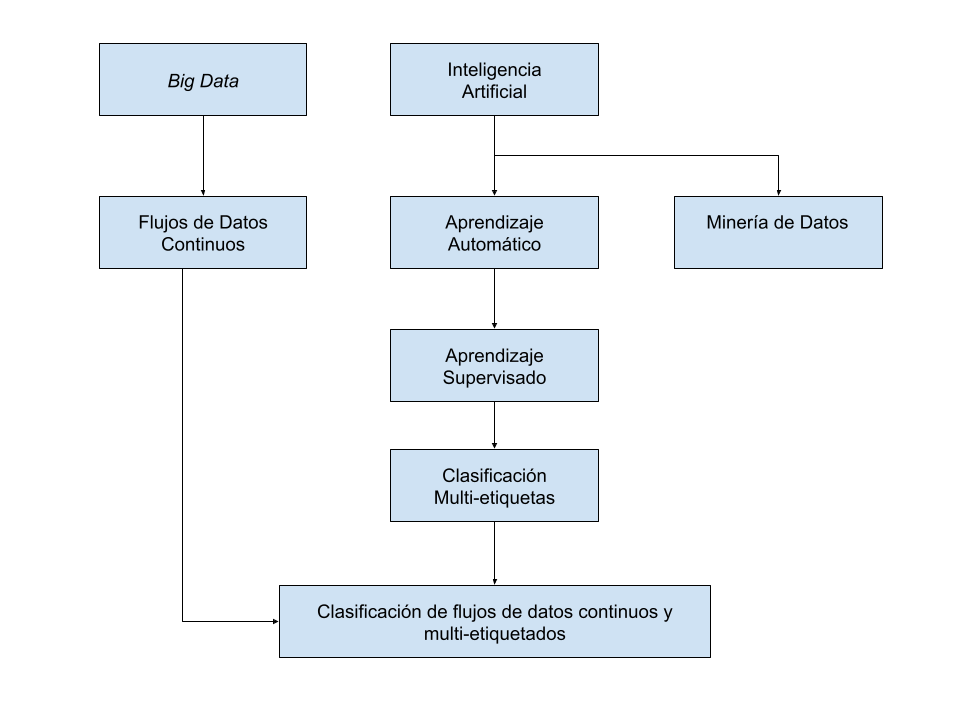
\includegraphics[width=.9\linewidth]{figures/study_field_taxonomy_v2.png}
   \centering
   \caption{Taxonomía del campo de estudio.}
   \label{fig:campo_estudio}
\end{figure}

En pocas palabras, el presente trabajo de investigación se enmarca en las áreas
de \textit{big data} y minería de datos, con aplicación en escenarios de
\textit{streaming} o flujos continuos de datos y abordando clasificaciones
multi-etiquetas. También se aprovechan técnicas del área de procesamiento de
lenguaje natural para tratar corpus de texto libre y extraer \textit{features} o
características representativas de los datos.

La figura \ref{fig:campo_estudio} es un esquema que ilustra la taxonomía del
campo de estudio y la interrelación entre las áreas de investigación
involucradas.

\section{Aprendizaje Automático}

El aprendizaje automático, también conocido por su término en ingles
“\textit{Machine Learning}”, se enmarca dentro del área de la \acrfull{ia} y
estudia cómo las computadoras pueden “aprender” o mejorar su rendimiento
meramente a partir de datos y sin la intervención de un ser humano.  La idea
detrás de esta disciplina es lograr reconocer patrones subyacentes en los datos
y tomar decisiones en base a estos. Por ejemplo, un problema de aprendizaje
automático es el de reconocer dígitos escritos a mano a partir de un conjunto de
ejemplos (ver figura \ref{fig:reconocimiento_digitos}).  Aquí se tienen un
conjunto de imágenes, cada una representando un dígito del 0 al 9, y el objetivo
es construir un modelo que sea capaz de detectar de qué dígito se trata. Otro
ejemplo es el de hallar documentos de texto que son relevantes a una consulta
del usuario. En este caso el modelo recibe un conjunto acotado de términos, los
cuales describen una necesidad de información del usuario, y el modelo debe ser
capaz de retornar los documentos que satisfacen la consulta.  

Estos problemas se suelen categorizar en aprendizaje supervisado o no
supervisado, de acuerdo a si se conoce o no de antemano el concepto o etiqueta
que define a los datos. Se desarrollará más sobre este punto en las próximas
secciones. De entre los problemas de aprendizaje supervisado se destaca aquí el
de clasificación, el cual será descrito a continuación.

\begin{figure}
   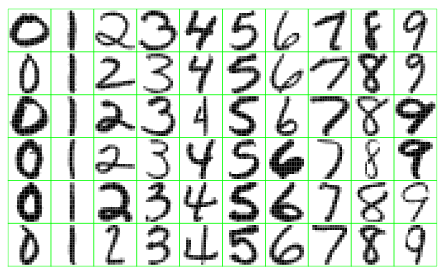
\includegraphics[width=0.66\linewidth]{figures/digits_recognition_v2.png}
   \centering
   \caption{Dígitos escritos a mano. Fuente: \citetitle{hastie_elements_2009}
   (\citeyear{hastie_elements_2009}).}
   \label{fig:reconocimiento_digitos}
\end{figure}

\section{Clasificación}

\subsection{Definición}
\label{clasificacion}

La clasificación es una tarea de minería de datos muy popular que consiste en
hallar modelos que describen la o las clases intrínsecas de los datos. La clase
corresponde a un concepto que representa al dato y es una etiqueta categórica,
es decir, un valor discreto de entre un conjunto de valores previamente
conocidos. Estos modelos, también llamados clasificadores, son capaces de
predecir la clase a la que corresponden datos previamente desconocidos. Por
ejemplo, se puede construir un modelo de clasificación para categorizar nuevos
correos electrónicos  de acuerdo a si se trata de correo basura (también
conocido como "\textit{spam}") o no. Dicho análisis puede ayudar a obtener un
mayor entendimiento de los datos a alto nivel. Las tareas de clasificación han
sido aplicadas en áreas tales como las de aprendizaje automático, reconocimiento
de patrones o estadística. En un principio, buena parte de los algoritmos se
ejecutaban en memoria, con la limitación de espacio de almacenamiento que eso
conlleva. Investigaciones más recientes han desarrollado técnicas para escalar
los algoritmos de tal manera que puedan manejar datos de mayor tamaño, alojados
en memoria, en disco o procesados bajo demanda. Las aplicaciones para este tipo
de tareas son numerosas y entre ellas se encuentran las de detectar fraudes o
realizar diagnósticos médicos, entre otras.

La clasificación de datos consta de dos etapas, una de aprendizaje y otra de
clasificación o predicción. Durante la tarea de aprendizaje se construye el
modelo de clasificación  el cual describe un determinado número de clases o
conceptos. También se conoce esta etapa como la de entrenamiento ya que se
selecciona un subconjunto de los datos, llamado conjunto de entrenamiento, que
consta de instancias o tuplas seleccionadas aleatoriamente y con una o más
etiquetas asociadas. Formalmente, el problema de clasificación puede ser
formulado de la siguiente manera. Se recibe un conjunto etiquetado de
instancias, tupas o ejemplos de la forma $( X, y )$ donde cada tupla es un
vector $X=(x_{1},x_{2},\dots,x_{n})$, siendo cada valor una característica
distintiva, atributo o feature de la instancia. El vector $y$ por su parte toma
un valor de entre $n$ clases diferentes.

Este tipo de tareas se engloban dentro del campo de aprendizaje supervisado ya
que para cada instancia la etiqueta es conocida de antemano, y es aprovechada
para guiar o, siguiendo la metáfora, “supervisar” el aprendizaje del
clasificador. Esta es la diferencia principal contra algoritmos de aprendizaje
no supervisado, en los cuales la etiqueta no es conocida y se deben aplicar
técnicas para salvar esta restricción.

La primera etapa de una clasificación puede ser vista también como el
aprendizaje de una función $y=f(X)$ que pueda predecir la clase $y$ para una
tupla $X$. Por ejemplo, $X$ podría ser un mensaje de correo y la etiqueta $y$ la
decisión de si se trata de un correo basura o no. Desde esta perspectiva
queremos aprender una función que sea capaz de distinguir las clases
subyacentes.  Usualmente, esta asociación es llevada a cabo por algoritmos de
aprendizaje, los cuales internamente usan funciones matemáticas o reglas de
decisión. Algunos ejemplos de este tipo de algoritmos son los árboles de
decisión, \textit{naive} bayes, perceptrón, entre otros.

En la segunda etapa el modelo es usado para clasificar. En primer lugar, se
calcula una métrica de evaluación, tal como la exactitud o \textit{accuracy}.
Durante la etapa de entrenamiento esta estimación puede ser imprecisa, tomando
un valor que tiende a ser “optimista” o que da un valor de exactitud mayor al
rendimiento real. Esto sucede porque el clasificador puede llegar a incorporar
anomalías particulares en el conjunto de datos de entrenamiento. Este fenómeno
es llamado sobreajuste u “\textit{overfit}” y una técnica para reducirlo es
separar de entre los datos un subconjunto de prueba o de \textit{testing} que no
se usa durante el entrenamiento y a partir del cual se realizan predicciones y
se calculan las métricas de evaluación. En este contexto, la tarea de evaluación
es fundamental ya que es la vía a partir de la cual se determina qué algoritmos
o técnicas son más apropiados que otros para un problema en particular. Además
provee la información necesaria para corregir o ajustar los parámetros de los
algoritmos y así obtener modelos más robustos.

En definitiva, ambos pasos se aplican consecutivamente con el objetivo de lograr
hallar un modelo capaz de predecir etiquetas en instancias nuevas y
desconocidas.

\subsection{Algoritmos}
\label{clasificacion_algoritmos}

Como se mencionó en la sección anterior, una de las etapas de clasificación
consiste en generar un modelo capaz de clasificar instancias desconocidas. En
esta etapa se pueden aplicar diversos tipos de algoritmos de acuerdo a la
naturaleza de la tarea en particular que se desea abordar. A continuación se
describen algunos algoritmos para generar modelos y que son particularmente
relevantes para este trabajo de investigación.

\subsubsection{\textit{Naive} Bayes}

\textit{Naive} Bayes es un modelo de clasificación computacionalmente simple
pero cuyo rendimiento es competitivo contra otros modelos más complejos. Se dice
que es un clasificador estadístico ya que se basa en el teorema de Bayes. La
idea es computar una probabilidad para cada una de las clases, basada en los
atributos de la instancia y seleccionar aquella de mayor probabilidad. El
término “\textit{naive}” es el inglés para el término “\textit{ingenuo}” y nace
de la presunción que hace el algoritmo de que los atributos son independientes
entre sí, o condicionalmente independientes. Esta presunción raramente se cumple
en los escenarios donde se aplica pero contribuye a su simplicidad computacional
y a su velocidad durante el entrenamiento.

El teorema de Bayes se define formalmente de la siguiente manera:

\begin{equation}
   P(H \mid X) = \frac{P(X \mid H) P(H)}{P(X)}
\end{equation}

En esta ecuación, el vector $X$ es una tupla definida tal como en la sección
anterior y en términos bayesianos representa la “evidencia”. $P(X)$, por lo
tanto, es la probabilidad de que la tupla contenga los atributos que posee. Por
su parte, $H$ es la hipótesis de que la tupla pertenece a una determinada clase
y $P(H)$ su probabilidad. Esta es conocida como probabilidad “a priori”. De la
misma manera, $P(H|X)$ es la probabilidad de que la hipótesis $H$ sea cierta
bajo la evidencia $X$. A esta se la llama probabilidad “a posteriori” con $H$
condicionada por $X$ y es el valor que se quiere determinar en una tarea de
clasificación.  Finalmente, $P(X|H)$ indica la probabilidad de que la tupla tenga
unos atributos determinados dado que se satisface la hipótesis.

Por su parte, la fórmula de \textit{Naive} Bayes es similar:

\begin{equation}
   P(C_{i} \mid X) = P(X \mid C_{i}) P(C_{i})
\end{equation}

Aquí el término $P(X)$ es descartado ya que se asume constante para todas las
clases. La hipótesis $H$ es representada como $C_{i}$ que es un valor de la
tupla $C=(C_{1},C_{2},\dots,C_{m})$, donde $m$ es el número de clases. La
presunción “ingenua” es aplicada para el cálculo del término $P(X \mid C_{i})$
gracias a lo cual se puede definir de la siguiente manera:

\begin{equation} 
   P(X \mid C_{i}) = \prod\limits_{k=1}^n{P(x_{k} \mid C_{i})} =
   P(x_{1} \mid C_{i}) \times 
   P(x_{2} \mid C_{i}) \times \dots, \times 
   P(x_{n} \mid C_{i})   
\end{equation}

Finalmente, el modelo seleccionará la clase que maximice el valor de
probabilidad.  

Como se ha dicho anteriormente, la simplicidad, velocidad computacional y su
competitividad en métricas de exactitud hacen de \textit{Naive} Bayes un
algoritmo destacado en el campo de aprendizaje automático
\cite{wickramasinghe_naive_2020} y ha sido aplicado para problemas diversos,
tales como el de hallar errores en programas de computación
\cite{arar_feature_2017}, predecir enfermedades del corazón
\cite{dulhare_prediction_2018} o detectar ataques en una red de computadoras
\cite{kalutarage_detecting_2015}.


\subsubsection{Árboles de Decisión}

Los árboles de decisión son un modelo de clasificación que se destaca por ser de
fácil interpretación e intuitivo para el ser humano. De hecho, se puede generar
una representación gráfica del árbol generado para asistir a la comprensión del
del modelo y de cómo se comporta durante una predicción. En cuanto a su
estructura, un árbol de decisión contiene nodos, cada uno representando un
atributo de la colección. Estos nodos se conectan con otros nodos a partir de
enlaces o “ramas” que representan un valor o un rango de valores de ese
atributo. Los nodos de menor jerarquía son llamados “hojas” y contienen la clase
de la predicción, y el nodo de mayor jerarquía es llamado “raíz”. Al momento de
predecir una instancia nueva, la clasificación se realiza de la siguiente
manera:  se toma la instancia nueva, la cual no tiene una etiqueta asociada, y
los valores de sus atributos son comparados contra los del árbol, luego se traza
un camino desde el nodo raíz hasta la hoja que contiene una clase y dicha clase
es la predicción resultante. 

Los árboles de decisión se generan a partir de un algoritmo de inducción.
Existen varios de estos algoritmos pero todos son variantes que han sido
diseñadas bajo un misma principio: construir  el árbol de una manera
“voraz”\footnote{Se le llama voraz o \textit{greedy} a un algoritmo que busca
   hallar la opción óptima en cada paso y, de esta manera, alcanzar la solución
   general óptima para resolver un problema.  Esto lo diferencia de algoritmos
   como los de \textit{backtracking}, los cuales exploran distintas
posibilidades y pueden volver al inicio en búsqueda de una mejor solución},
comenzando desde el nodo raíz (conocido como enfoque \textit{top-down}) y
eligiendo en cada paso el atributo más informativo o que maximice alguna medida
de ganancia de información. 

Algunos de estos algoritmos son:

\begin{description} 

   \item[\acrshort{id3}] Son las siglas de \textit{\acrlong{id3}} y fue
      desarrollado en 1986 por Ross Quinlan. Consiste en crear un árbol de
      múltiples vías, buscando para cada nodo el atributo categórico que lance
      la mayor ganancia de información para las clases categóricas. Los árboles
      crecen en un tamaño máximo y luego se realiza el paso de poda para mejorar
      el poder de generalización del modelo sobre datos desconocidos.

   \item[C4.5] Es la evolución del algoritmo \acrshort{id3}. La principal mejora
      con respecto a su predecesor es que elimina la restricción de que los
      atributos deban ser categóricos. Esto lo consigue particionando el valor
      continuo en rangos o en un conjunto de intervalos discretos. C4.5
      convierte el árbol entrenado en conjuntos de reglas de decisión. 

   \item[\acrshort{cart}] Son las siglas de \acrlong{cart} y es un algoritmo muy
      similar al C4.5 pero que soporta clases numéricas, lo cual permite
      resolver problemas de regresión. 

\end{description}

Una tarea fundamental en la generación de un árbol es definir un criterio de
división para seleccionar el mejor atributo en cada paso. Existen diversas
técnicas para abordarla, una de ellas es la de “Ganancia de Información”, usada
por el algoritmo \acrshort{id3}. La Ganancia de información busca seleccionar el
atributo que posee mayor variabilidad o representatividad de los datos y se
sustenta en el cálculo de la entropía o medida de desorden. La idea de fondo es
hallar el atributo que reduzca la entropía esperada. La entropía en el conjunto
de datos $D$ se calcula de la siguiente manera:

\begin{equation}
   Entropia(D) = - \sum_{i=1}^{m} p_{i}\log_{2}(p_{i})
\end{equation}

Aquí $p_{i}$ corresponde a la probabilidad de que una tupla de $D$ corresponda a
la clase $C_{i}$.  

Luego, la ganancia de información es:

\begin{equation}
   Ganancia(A) = Entropia(D) 
   - \sum_{j=1}^{v} \frac{\left\| D_{j} \right\|}{\left\| D \right\|} 
   \times Entropia(D_{j})
\end{equation}

Aquí el atributo $A$ divide al conjunto de datos en $v$ particiones, siendo $v$
los valores posibles que toma $A$. $D_{j}$ es el subconjunto de los datos cuyas
tuplas poseen el valor $v$ del atributo $A$, siendo $\left\|D_{j}\right\|$ su
cardinalidad o número de instancias del subconjunto. Al dividir este término por
la cardinalidad del conjunto de datos, se obtiene un valor que representa el
peso de la partición y es aplicado sobre la entropía esperada.

Una vez obtenidos los valores de ganancia para cada atributo, se selecciona
aquel que maximiza la ganancia y este será el criterio de separación en el nodo.

El algoritmo C4.5 introdujo una mejora en esta técnica llamada “Razón de
Ganancia”. La misma busca disminuir uno de los efectos adversos que provoca la
técnica de ganancia de información, esta es, que tiende a favorecer a atributos
con un mayor número de valores posibles. La razón de ganancia, en primer lugar,
reemplaza la fórmula $Entropia(D)$ por la siguiente:

\begin{equation}
   EntropiaRG_{A}(D) = - \sum_{j=1}^{v} \frac{\left\| D_{j} \right\|}{\left\| D \right\|} 
   \times \log_{2}(\frac{\left\| D_{j} \right\|}{\left\| D \right\|})
\end{equation}

A su vez, el nuevo cálculo de la ganancia se formula así:

\begin{equation} \label{eq:gan_c45}
   RazonGanancia(A) = \frac{Ganancia(A)}{EntropiaRG_{A}(D)} 
\end{equation}

Finalmente, el atributo de mayor razón de ganancia es seleccionado.

\todo[inline]{Aplicaciones de árboles de decisión en la literatura}

\todo[inline]{Figura de un árbol}

\todo[inline]{Subsección para sgd?, svm?, perceptrones?}

\subsubsection{Ensambles}

Los ensambles son un conjunto de clasificadores que, al ser combinados, pueden
realizar mejores predicciones que cualquiera de ellos individualmente. En pocas
palabras, el enfoque de ensambles consiste en generar $k$ clasificadores, de un
mismo tipo o no, y entrenarlos con subconjuntos de la colección de entrenamiento
original. Dada una tupla nueva, cada clasificador devuelve su propia predicción,
llamada “voto” y luego el ensamble devuelve la predicción final basada en esos
votos.

La aplicación de ensambles en problemas de clasificación nace de la
imposibilidad de generar un único modelo capaz de generalizar lo suficiente como
para lograr un rendimiento perfecto. Ante la presencia de datos ruidosos,
atípicos o erróneos los clasificadores pueden tender a clasificar mejor para un
subconjunto de datos y no tan bien para otros. Este escenario es aprovechado por
el enfoque de ensambles ya que su éxito tiene correlación con la existencia de
diversidad en la clasificación, esto es, que haya variabilidad entre los
subconjuntos de datos, modelos o hiper-parámetros, entre otros factores. A mayor
esta diversidad, los errores particulares de un ensamble se aíslan y serán
filtrados por la clasificación final. Como resultado se espera una disminución
del error total de la clasificación así como también una mayor exactitud en la
predicción, comparando contra los clasificadores base. Por otro lado, un enfoque
de ensambles abre la posibilidad de distribuir y/o paralelizar el cómputo de la
predicción, pudiendo así mejorar los tiempos de ejecución durante el
entrenamiento.

Existen distintos tipos de ensamble, de acuerdo a su construcción y
arquitectura. A continuación se describen 3 de ellos: los ensambles de tipo
\textit{bagging}, los de tipo \textit{boosting} y los de tipo \textit{stacked}. 

\begin{description} 

   \item[Bagging] Esta es una de las primeras técnicas de ensambles conocidas y
      fue introducida por
      \citeauthor{breiman_bagging_1996}\cite{breiman_bagging_1996}. La misma se
      desarrolla de la siguiente manera: dado un conjunto de entrenamiento $D$
      con $n$  tuplas, \textit{bagging} genera un número $m$ de nuevos conjuntos
      de datos de entrenamiento, cada uno con $n$ tuplas. Para esto se toman
      tuplas del conjunto original de manera aleatoria y con reemplazo, es decir
      que puede haber tuplas repetidas y otras que no están incluidas en el
      nuevo conjunto.  Luego a partir de cada conjunto nuevo, se entrena un
      clasificador $M_{i}$. Cada clasificador puede ser del mismos tipo ya que
      la diversidad está dada por los datos. En la etapa de clasificación, cada
      modelo $M_{i}$ genera una predicción que cuenta como un voto. El ensamble
      cuenta los votos y elige la clase con mayor cantidad de votos, siendo esta
      la decisión final del ensamble.


   \item[Boosting] En la técnica de \textit{boosting} se asigna un peso a cada
      tupla de entrenamiento y se generan un conjunto de clasificadores, uno
      luego del siguiente. A diferencia del método de \textit{bagging},
      \textit{boosting} trabaja siempre sobre el mismo conjunto de datos y la
      variabilidad está dada por los pesos que son asignados. El proceso es el
      siguiente: para el primer modelo de clasificación, $M_{i}$, los pesos son
      inicializados en un mismo valor para todas las tuplas. Una vez que se
      entrena este modelo, los pesos son actualizados de tal manera que el
      siguiente clasificador $M_{i} + 1$ trate de manera particular a las tuplas
      mal clasificadas por Mi, de tal manera de llegar a una clasificación
      correcta.  El clasificador final combina los votos de cada clasificador
      individual , donde el peso del voto de cada clasificador es una función de
      su exactitud. 


   \item[Stacking] Stacking es una técnica desarrollada por
      \citeauthor{wolpert_stacked_1992}\cite{wolpert_stacked_1992} y consiste en
      entrenar un nuevo clasificador de acuerdo a las predicciones realizadas
      por otros modelos, tomando la salida de estos modelos como entrada, de tal
      manera de lograr hallar una combinación que produzca una mejor predicción.
      Este tipo de ensambles puede ser visto como un conjunto de capas. La
      primera capa consta de un ensamble de clasificadores que aprenden a partir
      de los datos de entrenamiento. Esta capa no necesariamente usa
      clasificadores del mismo tipo, mismos hiper-parámetros o particiones de la
      colección iguales, quedando estos detalles a cargo de quien diseña esta
      capa. La siguiente capa es el clasificador individual, o
      meta-clasificador, que se alimenta de las salidas de los clasificadores de
      la capa inferior y realiza el aprendizaje a partir de las clases
      producidas por estas salidas y las clases reales.

\end{description}

Una de las tareas a tener en cuenta durante el entrenamiento de un ensamble es
la de combinar las salidas de cada modelo en una salida final. La estrategia más
común y simple es la de mayoría de voto, aplicada por los métodos de
\textit{bagging}, pero existen múltiples y no necesariamente un ensamble de tipo
\textit{bagging} debe aplicar esta estrategia. Por ejemplo, algunos
clasificadores pueden decidir producir una salida sólo en el caso de que más de
la mitad de ellos coincidan, o incluso ser más restrictivos y obligar a que la
coincidencia sea total. El enfoque de \textit{boosting} por su parte, pondera al
voto de acuerdo a los pesos que calcula, dando predominio a determinadas
instancias.  También se suele dar un mayor peso a determinados clasificadores
por sobre otros. Este tipo de métodos se los denomina “mayoría de voto
ponderada” y pueden llevar a un rendimiento superior.

\todo[inline]{Aplicaciones de ensambles en la literatura}

\todo[inline]{Figura de ensamble}

\section{Clasificación Multi-etiquetas}

A diferencia del aprendizaje automático tradicional, que usa datos de etiqueta
única para representar objetos del mundo real, cada instancia en el aprendizaje
multi-etiquetas representa un único objeto pero puede contener más de una
etiqueta. Por consiguiente, la tarea de clasificación consiste hallar una
función que logre asignar a cada objeto, nuevo y desconocido, el conjunto de
etiquetas que lo caracteriza.

En este apartado se da una definición formal, se detallan las características de
un conjunto de datos multi-etiquetados y se  describen algunos métodos
tradicionales de clasificación multi-etiquetas junto con sus ventajas,
desventajas, aplicaciones y motivaciones.

\subsection{Definición Formal y Métricas}

Asumiendo que $X=\mathbb{R}^{d}$ denota el espacio de instancias $d$
dimensional, y que $Y = \{y_{1}, y_{2}, \dots, y_{q}\}$ denota el espacio de
etiquetas con $q$ etiquetas posibles, la tarea de clasificación multi-etiquetas
consiste en entrenar un conjunto $D = \{(x_{i}, Y_{i}) \mid 1 \leq i \leq m\}$
para hallar una función $h$ tal que $h: X \rightarrow 2^y$. A su vez, $X_{i}$ es
un vector de atributos $d$ dimensional definido como $(x_{i1}, x_{i2}, \dots,
x_{id})$. $Y_{i}$, por su parte, es el conjunto de etiquetas sociadas a la
instancia $X_{i}$. Luego, para cada instancia desconocida $X \rightarrow X$ el
clasificador $h$ predice $h(x) \subseteq Y$ que representa el conjunto de
etiquetas hallado para $x$.

A su vez, se definen un conjunto de métricas que describen el grado de
multi-etiquetado que tiene un conjunto de datos dado, o en otras palabras, hasta
qué punto cada ejemplo posee más de una etiqueta. Algunas de ellas son: 

\begin{description}
   \item{Cardinalidad de etiquetas}: Es el promedio de etiquetas por instancia
      del conjunto de datos. Se define como: 
      \begin{equation}
         CardE(D) = \frac{1}{m} \sum_{i=1}^{m} \left\|Y_{i}\right\|
      \end{equation}
      Por lo tanto, a mayor el valor de cardinalidad, mayor es el número de
      etiquetas de una instancia. Por ejemplo, si $CardE = 1$, entonces la
      mayoría de ejemplos tiene una única etiqueta y, por consiguiente, se puede
      decir que la colección tiene un grado bajo de multi-etiquetado.  
   \item{Densidad de etiquetas}: Es la cardinalidad de etiquetas normalizada al
      número total de etiquetas de $D$ y se define como:
      \begin{equation}
         DenE(D) = \frac{CardE(D)}{\left\|Y\right\|}
      \end{equation}
      Así pues, un valor alto de densidad significaría que cada instancia puede
      ser una buena representación de las etiquetas del conjunto. De la misma
      manera, un valor bajo suele implicar dispersión, esto es, que la mayoría
      de las instancias tienen un subconjunto acotado de las etiquetas. 
   \item{Diversidad de etiquetas}: Es el número de conjuntos de etiquetas
      unívocos que aparecen en instancias de $D$. Se define como:
      \begin{equation}
         DivE(D) = \left\|\{Y \mid \exists x: (x, Y) \in D\}\right\|
      \end{equation}
      Aquí la interpretación es que, a mayor el valor de diversidad, menor es la
      constancia con la que las etiquetas aparecen en las instancias. De manera
      similar a la cardinalidad, el valor de diversidad también puede
      normalizarse por el número de instancias del conjunto de datos: 
      \begin{equation}
         DivEProm(D) = \frac{DivE(D)}{\left\|D\right\|}
      \end{equation}
\end{description}

\subsection{Algoritmos}

Como se había anticipado en la sección \ref{intro_mll}, la tarea de aprendizaje
sobre datos multi-etiquetados puede ser encarada siguiendo dos grandes enfoques,
llamados “Transformación del Problema” y “Adaptación del Algoritmo”. A
continuación se describen ambos enfoques y algunos de sus algoritmos más
representativos.

\subsubsection{Transformación del Problema} 

Esta categoría engloba al conjunto de algoritmos que abordan el problema de
clasificación multi-etiquetas transformándolo en múltiples problemas de
clasificación de única etiqueta, lo cual permite aplicar algoritmos de
clasificación convencionales. Tres de estos métodos son particularmente
relevantes para este trabajo: “\acrfull{br}”, “\acrfull{cc}” y “\acrfull{lp}”.

\paragraph{\acrfull{br}}

El algoritmo de Relevancia Binaria, conocido como \textit{\acrlong{br}} en la
literatura, es un enfoque que consiste en descomponer la tarea de clasificación
\acrshort{mll} en $\left\|q\right\|$ clasificadores binarios, independientes y
de etiqueta única.  A partir de esta transformación se puede seleccionar
cualquier algoritmo de clasificación como clasificador base del problema (ver
los algoritmos presentados en la sección \ref{clasificacion_algoritmos}).  Cada
clasificador binario $g_{j}$ es entrenado con todas las instancias de la
colección pero incluyendo solo la etiqueta $j$, la cual se activa o desactiva de
acuerdo a si es relevante a la instancia. Luego la predicción de una instancia
desconocida se realiza combinando las salidas de cada clasificador individual,
esto es: 

\begin{equation}
   Y = {y_{j} \mid g_{j}(x) > 0, 1 \leq j \leq q}
\end{equation}
 
Llegado el caso en que ninguno de los clasificadores retornen etiquetas activas,
el conjunto $Y$ será vacío.

Este enfoque se dice que es de primer orden (ver sección \ref{estrategias_mll})
y no tiene en cuenta la correlación o interdependencias entre etiquetas. Este es
uno de los principales inconvenientes de este algoritmo ya que, en este tipo de
problemas de \acrshort{mll}, es usual hallar que determinadas etiquetas se
activan en conjunto con mayor probabilidad. Pese a ello, \acrshort{br} es un
enfoque muy utilizado \cite{zhang_review_2014} ya que es simple de implementar,
intuitivo y computacionalmente poco costoso en comparación con algoritmos que sí
tienen en cuenta la relación entre etiquetas.  

\paragraph{\acrfull{cc}}

Las cadenas de clasificadores o \textit{\acrlong{cc}}
\cite{read_classifier_2011} es una técnica que convierte el problema de
\acrshort{mll} en una ”cadena” de problemas de clasificación binaria, tal que el
siguiente clasificador de la cadena posee las predicciones de los anteriores. En
principio, la división del conjunto de datos es similar a la que se hace en el
enfoque anterior, designando un clasificador por cada etiqueta. Durante el
entrenamiento el clasificador inicial, seleccionado aleatoriamente, usa de
entrada los atributos originales, tal como el clasificador \acrshort{br}. Luego
la salida de este clasificador es añadida al espacio de atributos como un
atributo más de cada instancia, para que posteriormente, estos atributos sean la
entrada del siguiente clasificador, el cual también es seleccionado al azar.
proceso es repetido hasta completar todos los clasificadores.  Como se ve se
produce un ”encadenamiento” de clasificadores que no es accidental y tiene como
fin conservar la dependencia entre etiquetas, ya que cada clasificador logra
capturar la correlación entre las etiquetas de los anteriores clasificadores. 

Cabe notar que en esta técnica cobra especial importancia el ordenamiento de los
clasificadores ya que este orden tiene un impacto directo sobre el resultado de
la predicción. En otras palabras, si el ordenamiento de clasificadores se
modifica, el modelo final otorgará resultados diferentes. Para salvar esta
dificultad se han propuesto modelos como el de \acrfull{ecc}. El mismo genera un
conjunto de modelos de \acrshort{cc} con distintos ordenamientos y entrenados
con diversos subconjuntos de datos, generados con reemplazo o no. Durante la
predicción, cada cadena produce un conjunto de etiquetas, que son los votos, y
la salida final será computada por un algoritmo que combine cada salida
individual.
 
\paragraph{\acrfull{lp}}

El conjunto de potencias de etiquetas o \textit{\acrlong{lp}}
\cite{tsoumakas_random_2011} es una técnica que se encarga de transformar el
problema de \acrshort{mll} en uno de clasificación multi-clase, de tal manera de
poder abordarlo con algoritmos de este tipo. La clasificación multi-clase es un
enfoque usado para tratar con ejemplos en donde la etiqueta es única pero cuenta
con más de dos clases. Un ejemplo de este tipo de problemas es el de análisis de
sentimiento de texto, en donde las clases pueden ser “positivo”, “negativo” y
“neutral”. 

En \acrshort{lp} cada etiqueta indica el subconjunto de etiquetas de
la instancia. Esto es beneficioso en cuanto a que se logra preservar la
dependencia entre etiquetas. Sin embargo, el modelo tiene algunas dificultades.
En primer lugar, el espacio de clases posibles es exponencial y su cantidad de
clases puede llegar a ser de $2^{\left\|L\right\|}$ como máximo. A su vez, pueden
llegar a arribar ejemplos con una combinación de etiquetas que el modelo no
recibió durante el entrenamiento, por lo cual no logra generalizar lo suficiente
y se lo considera un modelo incompleto. A fin de sobrepasar estas complicaciones
se desarrolló la técnica de Conjuntos Podados o \acrfull{ps}. La misma consiste
en preservar para la clasificación aquellos subconjuntos de etiquetas que son
más frecuentes en la colección, y eliminar los demás. Con esto se logra
disminuir considerablemente el espacio de clases y disminuye la complejidad
computacional, tanto durante el entrenamiento como durante la predicción.

\subsubsection{Adaptación del Algoritmo}

Además del enfoque de transformación del problema, otros autores abordan la
clasificación multi-etiquetas a partir de la adaptación de algoritmos clásicos y
bien conocidos. Esta categoría engloba al conjunto de algoritmos que abordan el
problema de \acrshort{mll} mediante la modificación de algoritmos de etiqueta
única para que sean capaces de manejar la nueva naturaleza de los datos en estas
tareas. Las modificaciones que se introducen pueden variar en complejidad según
el algoritmo tratado y las características de la colección.  Se han adaptado una
diversa cantidad de algoritmos incluyendo aquellos basados en redes neuronales,
árboles, métodos probabilísticos, entre otros \cite{herrera_multilabel_2016}.
Por mencionar algunos ejemplos, \citeauthor{gargiulo_deep_2018} usan redes
neuronales profundas para clasificar documentos de texto libre y comparan su
funcionamiento variando el número de etiquetas y aprovechando su estructura
jerárquica \cite{gargiulo_deep_2018}. Asimismo,
\citeauthor{tanaka_multi-label_2015} agregan al algoritmo de \acrshort{br} la
capacidad de capturar relaciones entre etiquetas a través del uso de árboles de
decisión y lo aplican en el área de la genómica \cite{tanaka_multi-label_2015}.

En lo que confiere a ambientes de flujos continuos de datos una de las técnicas
más populares en la literatura es la de Árbol de Hoeffding o
\textit{\acrfull{ht}} \cite{domingos_mining_2002}. A diferencia de los
algoritmos convencionales de árboles de decisión, \acrlong{ht} aborda los datos
de manera incremental. Así pues, en lugar de realizar decisiones de corte de
acuerdo a los datos previamente almacenados, \acrshort{ht} espera a tener una
cantidad suficiente de instancias para realizar el corte, con un cierto grado de
confianza. Esto significa que ya no es necesario guardar todos los datos de la
colección y que mantener una serie de estadísticas es suficiente para realizar
la clasificación. Otra de las propiedades a destacar de este método es que en
teoría se puede entrenar un árbol cuyo rendimiento se aproxime al generado en un
ambiente de \textit{batch}, con la suficiente cantidad de datos
\cite{bifet_machine_2018}. 

A partir de esto, y buscando sacar provecho de las ventajas mencionadas,
\citeauthor{read_scalable_2012} decidieron adaptar este algoritmo a problemas de
multi-etiquetas y desarrollaron el algoritmo llamado Árbol de Hoeffding
Multi-etiquetado o \textit{\acrfull{mlht}} \cite{read_scalable_2012}. Esto lo
consiguen a partir de rediseñar la fórmula de ganancia de información (ver
fórmula \ref{eq:gan_c45}) de tal manera de reflejar el impacto de todas las
clases a las cuales el ejemplo no pertenece. Desde que fue introducido en el año
\citeyear{read_scalable_2012}, \acrshort{mlht} ha sido usado como modelo de
comparación en reiteradas oportunidades \cite{sousa_multi-label_2018} y es uno
de los métodos más populares para atacar problemas de \acrshort{mll} en
ambientes de flujo continuo de datos.

Otro algoritmo muy popular para abordar este tipo de problemas y basado en
árboles de decisión incrementales es el llamado \acrshort{isoup} (siglas del
inglés \textit{\acrlong{isoup}}) \cite{osojnik_multi-label_2017}. El mismo fue
desarrollado inicialmente para hacer regresión de múltiples objetivos y luego
fue adaptado a tareas de \acrshort{mll}. Una de las novedades que introduce es
el uso de un perceptrón adaptativo en las hojas del árbol, lo cual le da la
versatilidad de poder trabajar tanto con problemas de clasificación como de
regresión.

\section{Clasificación de Flujos Continuos de Datos}

\section{Evaluación y Métricas}



\backmatter

%%%% GLOSARIO
\printglossary[type=\acronymtype]
\cleardoublepage

%%%% BIBLIOGRAFIA
\printbibliography

\end{document}
